Supppose we have
%\begin{multicols}{2}
\begin{itemize}
	\item binary columns $\bit{1}, \bit{2}$,
	\item counter-constant columns  \source{}, \targetOne{}, \targetTwo{}, $\targetOne{}\new{}$, $\targetTwo{}\new{}$,
	\item a counter-constant column \targetOne{}\mark{},
	\item byte columns \source{}\byte{}, \targetOne{}\byte{}, \targetTwo{}\byte{},
	\item accumulator columns $\acc{1}, \acc{2}, \acc{3}, \acc{4}$,
	\item a column \col{P},
	\item a ``counter column'' \ct{}.
		%\item[\vspace{\fill}]
\end{itemize}
%\end{multicols}
The interpreation is as follows:
\source{} is a limb from which we will harvest \emph{all} bytes (hence the descriptor \emph{full});
\targetOne{} and \targetTwo{} are limbs which we will updata using \source{}'s bytes;
$\targetOne{}\new{}$ and $\targetTwo{}\new{}$ are their ``new'' values;
\source{}\byte{}, \targetOne{}\byte{}, \targetTwo{}\byte{} are the respective byte decompositions;
\targetOne{}\mark{} is a marker for bytes in \targetOne{};
$\bit{1}$ plateaus at \targetOne{}\mark{};
$\bit{2}$ plateaus at $16 - \targetOne{}\mark{}$;
$\col{P}$ is pegged to $\bit{1}$ and builds the correct power of $256$ so that we may change the relevant prefix of \targetTwo{}.

The following collection of constraints ensures the desired behaviour.
% The interpreation of the greek letters ($\alpha'$, $\beta$, $\beta'$, $\gamma$) is given in \ob{TODO} figure~\ref{fig: one full to two}.
\begin{description}
	\item[Plateau constraints:]
		\begin{enumerate}
			\item $\plateau(\bit{1}, \targetOne{}\mark{}; \ct{})$
			\item $\plateau(\bit{2}, 16 - \targetOne{}\mark{}; \ct{})$
		\end{enumerate}
	\item[Prefix and suffix constraints:]
		\begin{enumerate}
			\item $\compSuffix(\acc{1}, \targetOne{}\byte{}, \bit{1}; \ct{})$, %i.e. $\acc{1}\implies\alpha'$,
			\item $\compPrefix(\acc{2}, \targetTwo{}\byte{}, \bit{1}; \ct{})$, %i.e. $\acc{2}\implies\beta$,
			\item $\compPrefix(\acc{3}, \source{}\byte{}, \bit{2}; \ct{})$, %i.e. $\acc{3}\implies\gamma$,
			\item $\compSuffix(\acc{4}, \source{}\byte{}, \bit{2}; \ct{})$, %i.e. $\acc{4}\implies\gamma'$,
		\end{enumerate}
	\item[Power constraint:] $\power(\col{P}, \bit{1}; \ct{})$,
	\item[Update constraints:] \If $\ct_{i} = \llargeMO$ \Then
		\begin{enumerate}
			\item $\targetOne\new_i = \targetOne_i + (\acc{3}_i - \acc{1}_i)$
			\item $\targetTwo\new_i = \targetTwo_i + (\acc{4}_i - \acc{2}_i) \cdot \col{P}_i$
		\end{enumerate}
\end{description}
We encapsulate all these constraints under a single relation
\[
	\oneFullToTwo
	\left( \begin{array}{c}
		\source{}, \targetOne{}, \targetTwo{}, \targetOne{}\new{}, \targetTwo{}\new{};\\
		\source{}\byte{}, \targetOne{}\byte{}, \targetTwo{}\byte{};\\
		\acc{1}, \acc{2},\\
		\acc{3}, \acc{4}, \col{P}; \\
		\targetOne{}\mark{}, \bit{1}, \bit{2}; \ct{};
	\end{array} \right)
\]

\begin{figure}[h!]
	\centering
	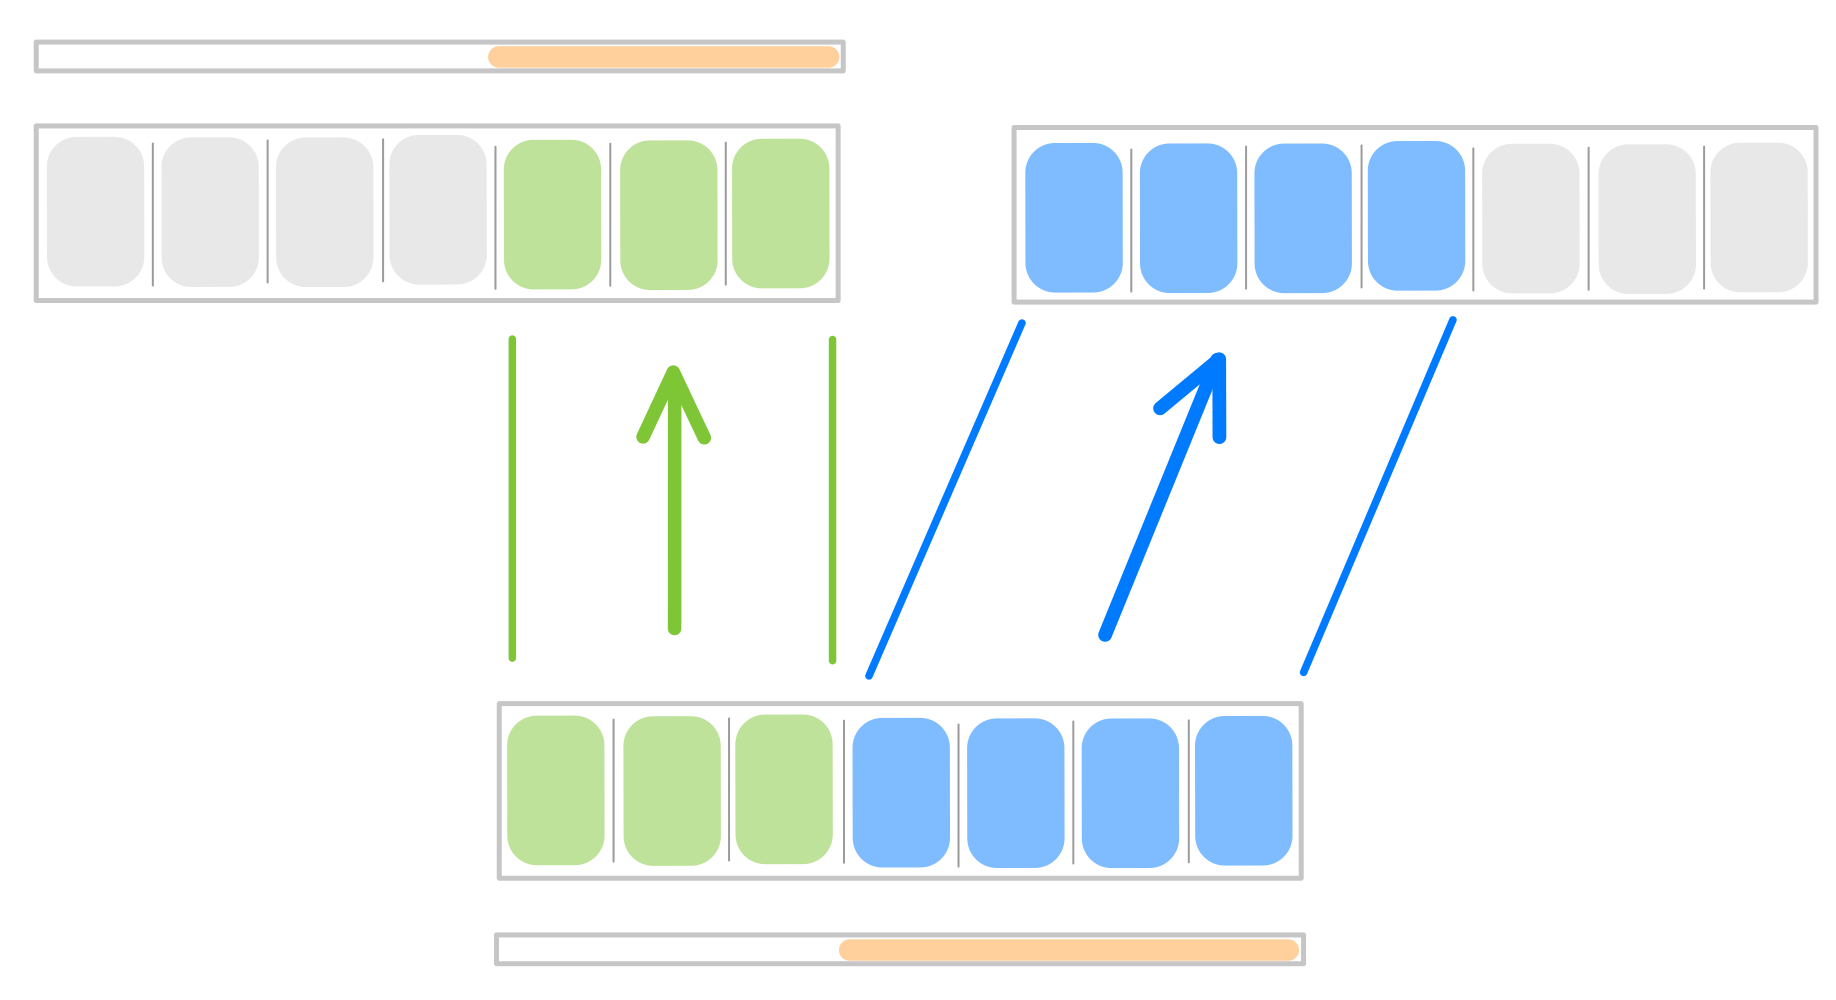
\includegraphics[width = 0.5\textwidth]{drawing/1_full_to_2}
	\label{fig: one full to two}
	\caption{This diagram explains the $\oneFullToTwo{}$ constraint and the greek letters mentioned in the constraints.}
\end{figure}
